\chapter{Datenmodellierung} % (fold)
\label{sec:datamodelling}
Um für das empirische Experiment eine Datenbasis zu schaffen, benötigt es ein Datenmodell. Hierbei soll ein möglichst realistisches und flexibles Modell genutzt werden, zudem sollte dieses Verzweigungen aufweisen um verschiedene Anfragekomplexität abbilden zu können. In diesem Szenario (vgl. Abb. 4.1) handelt es sich um ein Projektmanagement-Tool. Es existieren drei Klassen, welche über drei Beziehungen miteinander verbunden sind. Die Klasse \texttt{Person} modelliert einen Menschen, mit den Attributen \texttt{Firstname, Lastname, E-Mail}. Sie steht mit der Klasse \texttt{Project} in einer n:n-Beziehung, wodurch mehrere 

\noindent
\texttt{Project} Objekte zu einer \texttt{Person} zugeordnet werden können, aber auch mehrere \texttt{Person} Objekte an einem \texttt{Project} arbeiten können. In der Klasse \texttt{Project} werden nur der \texttt{Title} und das \texttt{Date}, an welchem das \texttt{Project} erstellt wurde, gespeichert. Ein \texttt{Project} steht in einer 1:n-Beziehung zur Klasse \texttt{Issue}. Dadurch kann einem \texttt{Issue} nur ein \texttt{Project} zugeordnet werden, ein \texttt{Project} kann aber mehrere \texttt{Issue} Objekte beinhalten. \texttt{Issue} speichert Daten wie etwa den \texttt{Title}, das \texttt{Date} an dem das \texttt{Issue} erstellt wurde, den \texttt{State} und die \texttt{StateReason}. \texttt{Issue} besitzt eine n:n-Beziehung zu \texttt{Person}, wodurch ein \texttt{Issue} von mehreren \texttt{Person} Objekten bearbeitet werden kann und eine \texttt{Person} in mehreren \texttt{Issue} Objekten arbeiten kann.
\vspace{1cm}
\label{sec:datenmodell}
\begin{figure}[h!]
	\centering
	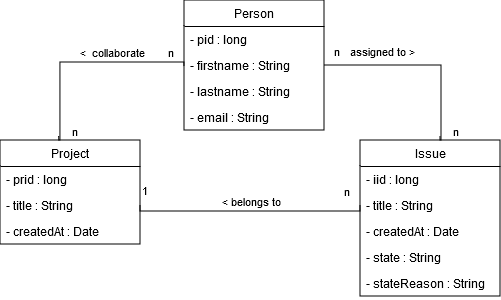
\includegraphics[scale=.8]{Illustrations/class_diagram.png}
	\caption{Klassendiagramm}
\end{figure}


% chapter datamodelling (end)

